\documentclass[12pt]{article}
\usepackage[margin=1in]{geometry}
\usepackage{amsmath}
\usepackage{graphicx}
\setlength{\parindent}{0pt}
% 使用系统字体,需要 XeLaTeX 或 LuaLaTeX 编译
\usepackage{fontspec}
\setmainfont{Times New Roman}
\usepackage{xcolor}
\newcommand{\avg}[1]{\left\langle #1 \right\rangle}
\newcommand{\doubleavg}[2]{\left\langle #1 \right\rangle\!\left\langle #2 \right\rangle}
\begin{document}

\title{Note for Scattering Amplitude Computation}
\author{Su Yingze}
\maketitle

\section{4-point case}
For the four point case $\mathcal{A}(V_2\Phi^\dagger V_1 \Phi )$, we can construct the color-ordered amplitude from the residue. First, we consider the $(+,-)$ helicity
configuration. There are two feynman diagrams contributing to the color-ordered amplitude.\\
\begin{figure}[htbp]
    \centering
    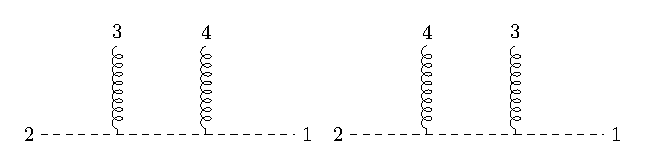
\includegraphics{4pt.eps}
    \caption{4pt.}
    \label{fig:myfigure}
\end{figure}

For the first diagram, the residue equals to
\begin{equation*}
    \mathcal{R}es|_{s_{12}=0}=\frac{[3 I ] [23]}{[I2]}\times \frac{\avg{I4}\avg{41}}{\avg{1I}}=\frac{\avg{24}[31]\avg{41}[23]}{[42]\avg{24}}
\end{equation*}
Similarly, the second one is
\begin{equation*}
    \mathcal{R}es|_{s_{13}=0}=\frac{\avg{4I}\avg{24}}{\avg{I2}}\times \frac{[31] [I3]}{[1I]}=\frac{\avg{24}[31]\avg{41}[23]}{\avg{32}[23]}
\end{equation*}

Then we can conclude that the four-point color-ordered amplitude $A[1,2,3^+,4^-]$ equals to
\begin{equation*}
    A[1,2,3^+,4^-]=\frac{\avg{24}[31]\avg{41}[23]}{\avg{32}[23][42]\avg{24}}=\frac{\avg{24}\avg{14}}{\avg{13}\avg{23}}
\end{equation*}

\textcolor{red}{$\star Bonus$}

It is still necessary to prove the color-ordered amplitude $A[1,2,3^+,4^+]$ equals to 0. Here we can use the color ordered Feynman rules to show the result.
\begin{equation*}
    A[1,2,3^+,4^+]\propto \frac{\left(\epsilon_3\cdot p_2\right)\left(\epsilon_4\cdot p_1\right)}{s_{23}}+\frac{\left(\epsilon_4\cdot p_2\right)\left(\epsilon_3\cdot p_1\right)}{s_{24}} 
\end{equation*}
Here we can utilize the spinor-helicity variable to express polarization vector
\begin{equation*}
    \epsilon_2^{+\mu}=\frac{\left <r_1|\gamma^\mu|3\right ]}{\sqrt{2}\avg{r_13}},\qquad \epsilon_4^{+\mu}=\frac{\left <r_2|\gamma^\mu|4\right ]}{\sqrt{2}\avg{r_24}}
\end{equation*}
here $r_1$ and $r_2$ represent the reference spinor.

We can freely choose $r_1=r_2=1$ or 2, then $\avg{r_1 2}$,$\avg{r_2 1}$,$\avg{r_1 1}$,$\avg{r_2 2}$, two of them equal to 0, so we can conclude that
\begin{equation*}
    A[1,2,3^+,4^+]=0
\end{equation*}
\section{5-point case}
For the 5-point case, we can utilize the BCFW recursion relation which can help us generate higher point amplitude from lower point on-shell subamplitudes. Here, 
we always consider the MHV (Maximal helicity violation) amplitude. 
\par
Let us begin with the simplest case $A[1,2,3_1^+,4_1^+,5_2^-]$, where the subscript represent which gauge group the particle belongs to. 
\end{document}